%============================================================
% Research Proposal — Reduction Ladder for Code & Mitigation
% Orange Innovation Labs — Submitted to Dr. Ghada
% Authors: Omar Abdelhamid, Nour Walid
% Compile with: pdflatex -> bibtex -> pdflatex x2
%============================================================
\documentclass[12pt, a4paper]{article}

%------------------------------------------------------------
% PACKAGES
%------------------------------------------------------------
\usepackage[T1]{fontenc}
\usepackage[utf8]{inputenc}
\usepackage{lmodern}
\usepackage{microtype}
\usepackage[left=2.5cm, right=2.5cm, top=3cm, bottom=3cm]{geometry}
\usepackage{xcolor}
\usepackage{graphicx}
\usepackage{amsmath, amssymb}
\usepackage{booktabs}
\usepackage{tabularx}
\usepackage{longtable}
\usepackage{array}
\usepackage{multirow}
\usepackage{fancyhdr}
\usepackage{titlesec}
\usepackage{tocloft}
\usepackage{hyperref}
\usepackage{enumitem}
\usepackage{mdframed}
\usepackage{tikz}
\usepackage{pgfplots}
\pgfplotsset{compat=1.18}
\usepackage{float}
\usepackage{caption}
\usepackage{subcaption}
\usepackage{setspace}
\usepackage{parskip}
\usepackage{soul}
\usepackage{pifont}
\usepackage{fontawesome5}
\usepackage{listings}
\usepackage{tcolorbox}
\tcbuselibrary{skins, breakable, listings}
\usepackage[backend=bibtex, bibstyle=ieee, citestyle=numeric-comp, sorting=none, maxbibnames=4]{biblatex}
\addbibresource{references.bib}

%------------------------------------------------------------
% ORANGE BRAND COLORS
%------------------------------------------------------------
\definecolor{OrangeMain}{RGB}{255, 100, 0}
\definecolor{OrangeDark}{RGB}{200, 70, 0}
\definecolor{OrangeLight}{RGB}{255, 165, 60}
\definecolor{DarkBG}{RGB}{20, 20, 25}
\definecolor{MidGray}{RGB}{80, 80, 90}
\definecolor{LightGray}{RGB}{240, 240, 245}
\definecolor{AccentBlue}{RGB}{30, 120, 200}
\definecolor{SuccessGreen}{RGB}{40, 160, 80}
\definecolor{AlertRed}{RGB}{200, 40, 40}

%------------------------------------------------------------
% HYPERREF SETUP
%------------------------------------------------------------
\hypersetup{
  colorlinks   = true,
  linkcolor    = OrangeDark,
  citecolor    = OrangeDark,
  urlcolor     = AccentBlue,
  pdftitle     = {Reduction Ladder for Code \& Multi-Arm Mitigation — Research Proposal},
  pdfauthor    = {Omar Abdelhamid, Nour Walid (Orange Innovation Labs)},
  pdfsubject   = {SLM Reasoning Evaluation and Multi-Arm Mitigation},
}

%------------------------------------------------------------
% SECTION HEADING STYLE
%------------------------------------------------------------
\titleformat{\section}
  {\large\bfseries\color{OrangeMain}}
  {\thesection.}{0.6em}{}
  [\color{OrangeMain}\titlerule]

\titleformat{\subsection}
  {\normalsize\bfseries\color{OrangeDark}}
  {\thesubsection.}{0.5em}{}

\titleformat{\subsubsection}
  {\normalsize\itshape\color{MidGray}}
  {\thesubsubsection.}{0.4em}{}

%------------------------------------------------------------
% HEADER / FOOTER
%------------------------------------------------------------
\pagestyle{fancy}
\fancyhf{}
\renewcommand{\headrulewidth}{0.5pt}
\renewcommand{\headrule}{\hbox to\headwidth{\color{OrangeMain}\leaders\hrule height\headrulewidth\hfill}}
\fancyhead[L]{\small\color{MidGray} Reduction Ladder for Code \& Mitigation}
\fancyhead[R]{\small\color{MidGray} Orange Innovation Labs}
\fancyfoot[C]{\small\color{MidGray} \thepage}
\fancyfoot[R]{\small\color{OrangeMain} \textbf{Confidential — Orange Restricted}}

%------------------------------------------------------------
% CUSTOM BOXES
%------------------------------------------------------------
\newtcolorbox{researchbox}[1][]{
  enhanced, breakable,
  colback=LightGray,
  colframe=OrangeMain,
  fonttitle=\bfseries\color{white},
  coltitle=white,
  attach boxed title to top left={yshift=-2mm, xshift=4mm},
  boxed title style={colback=OrangeMain, rounded corners},
  arc=3pt, boxrule=1pt,
  #1
}

\newtcolorbox{keybox}[1][]{
  enhanced, breakable,
  colback=DarkBG!5,
  colframe=OrangeDark,
  left=4pt, right=4pt,
  arc=2pt, boxrule=0.8pt,
  #1
}

\newtcolorbox{gapbox}{
  enhanced,
  colback=AlertRed!8,
  colframe=AlertRed,
  arc=3pt, boxrule=0.8pt,
  fonttitle=\bfseries,
  title={\faExclamationTriangle\ The Core Research Gap: The Memorisation Barrier},
  coltitle=AlertRed,
  attach boxed title to top left={yshift=-2mm, xshift=4mm},
  boxed title style={colback=white, colframe=AlertRed},
}

\newtcolorbox{noveltybox}{
  enhanced,
  colback=SuccessGreen!8,
  colframe=SuccessGreen,
  arc=3pt, boxrule=0.8pt,
  fonttitle=\bfseries,
  title={\faCheckCircle\ Our Novel Contribution: Diagnosis \& Multi-Arm Mitigation},
  coltitle=SuccessGreen,
  attach boxed title to top left={yshift=-2mm, xshift=4mm},
  boxed title style={colback=white, colframe=SuccessGreen},
}

%------------------------------------------------------------
% TOC STYLING
%------------------------------------------------------------
\renewcommand{\cftsecfont}{\bfseries\color{OrangeDark}}
\renewcommand{\cftsecpagefont}{\bfseries\color{OrangeDark}}
\renewcommand{\cftsubsecfont}{\color{MidGray}}
\setlength{\cftbeforesecskip}{4pt}

%------------------------------------------------------------
% LISTINGS (code style)
%------------------------------------------------------------
\lstdefinestyle{pythonstyle}{
  language=Python,
  basicstyle=\ttfamily\footnotesize,
  keywordstyle=\color{OrangeMain}\bfseries,
  commentstyle=\color{MidGray}\itshape,
  stringstyle=\color{SuccessGreen},
  numberstyle=\tiny\color{MidGray},
  numbers=left,
  stepnumber=1,
  breaklines=true,
  frame=single,
  rulecolor=\color{LightGray},
  backgroundcolor=\color{LightGray},
}

%============================================================
% DOCUMENT BEGIN
%============================================================
\begin{document}

%------------------------------------------------------------
% COVER PAGE
%------------------------------------------------------------
\begin{titlepage}
  \pagecolor{DarkBG}
  \color{white}
  \begin{center}
    \vspace*{1.5cm}
    
    % Orange bar
    {\color{OrangeMain}\rule{\textwidth}{3pt}}
    \vspace{0.4cm}
    
    {\Large\bfseries\color{OrangeLight} Orange Innovation Labs}\\[0.2cm]
    {\normalsize\color{MidGray} Research \& Advanced AI Division}
    
    \vspace{1.2cm}
    {\color{OrangeMain}\rule{0.4\textwidth}{1pt}}
    \vspace{1.2cm}
    
    {\Huge\bfseries\color{white}
      Reduction Ladder\\[0.3cm]
      \color{OrangeMain} for Code \& Mitigation}\\[0.5cm]
    
    {\large\color{LightGray}
      Probing and Resolving Pattern-Matching Collapse\\
      in Small Language Models via a\\
      Prioritized Multi-Arm Mitigation Framework}
    
    \vspace{1.5cm}
    {\color{OrangeMain}\rule{0.4\textwidth}{1pt}}
    \vspace{1.5cm}
    
    \begin{tabular}{rl}
      \textbf{\color{OrangeLight} Research Team:}  & \textbf{Omar Abdelhamid, Nour Walid}\\[4pt]
      \textbf{\color{OrangeLight} Submitted to:}   & Dr.\ Ghada — Research Supervisor\\[4pt]
      \textbf{\color{OrangeLight} Division:}        & Orange Innovation, AI Research Lab\\[4pt]
      \textbf{\color{OrangeLight} Document Type:}   & Technical Research Proposal\\[4pt]
      \textbf{\color{OrangeLight} Version:}         & 2.2 — Exhaustive Technical Specification\\[4pt]
      \textbf{\color{OrangeLight} Date:}            & August 2025\\[4pt]
      \textbf{\color{OrangeLight} Classification:}  & \textcolor{OrangeMain}{\bfseries Orange Restricted}\\
    \end{tabular}
    
    \vfill
    {\color{OrangeMain}\rule{\textwidth}{3pt}}
    \vspace{0.3cm}
    {\small\color{MidGray}
      This document contains confidential research material intended solely for\\
      internal review within Orange Innovation Labs.}
  \end{center}
\end{titlepage}

% Restore white background
\nopagecolor

%------------------------------------------------------------
% ABSTRACT
%------------------------------------------------------------
\newpage
\begin{researchbox}[title={Executive Abstract}]
Small Language Models (SLMs) in the 1--3B parameter range are essential for cost-efficient, on-device code generation across Orange Innovation's product stack (e.g., network automation, self-healing script generation, and developer productivity assistants). However, empirical studies reveal that these models often rely on superficial pattern matching rather than algorithmic reasoning, leading to catastrophic failure under mild prompt perturbations.

This proposal introduces a comprehensive, two-stage research framework:
\begin{enumerate}[leftmargin=1.5em]
  \item \textbf{Diagnostic Reduction Ladder (L0--L5):} Grounded in the peer-reviewed \textbf{EvoEval (EMNLP 2024)} benchmark suite, we map six progressive levels of algorithmic transformation to quantify the exact \emph{collapse point} ($\ell^*$) where model competence fails across lexical, syntactic, and contextual shifts.
  \item \textbf{Prioritized Multi-Arm Mitigation Framework:} Rather than confining our exploration to a single method, we formulate and empirically compare representative, state-of-the-art techniques across four distinct research paradigms:
  \begin{itemize}
    \item \textbf{Arm 1 (Priority 1 — Primary):} Invariance-Regularized Policy Optimization (\textbf{Inv-GRPO}) using cross-perturbation paired sampling and consistency rewards.
    \item \textbf{Arm 2 (Priority 2 — SFT Distillation):} Contrastive Thought-Template SFT (\textbf{Contrastive-SFT}) incorporating negative shortcut rejection traces.
    \item \textbf{Arm 3 (Priority 3 — Structural Syntax):} AST-Guided Structural Policy Optimization (\textbf{AST-RL}) utilizing syntax tree similarity metrics.
    \item \textbf{Arm 4 (Priority 4 — Process Verification):} Stepwise Execution-Gated RL (\textbf{Step-RLVR}) with fine-grained intermediate contract rewards.
  \end{itemize}
\end{enumerate}

We systematically evaluate all mitigation arms on \texttt{Qwen2.5-Coder-1.5B-Instruct}, delivering a robust empirical comparison, verified checkpoints, and actionable deployment guidelines for Orange.
\end{researchbox}

\vspace{0.5cm}
\tableofcontents
\newpage

%============================================================
\section{Introduction \& Motivation}
%============================================================

The deployment of Small Language Models (SLMs) in production software pipelines requires predictable algorithmic reliability. In telecommunications and enterprise infrastructure, code generation agents must synthesize resilient code even when user prompts deviate from canonical textbook phrasings.

\subsection{The Mimicry vs.\ Reasoning Crisis}

Current benchmarks (e.g., HumanEval, MBPP) suffer from severe data contamination and lexical saturation. A model achieving 85\% pass@1 on verbatim benchmark problems often experiences severe performance collapse when minor, semantics-preserving modifications are applied:
\begin{itemize}[leftmargin=1.5em]
  \item \textbf{Lexical Shifts:} Altering variable names or identifiers causes up to 30\% degradation~\cite{gsm_symbolic}.
  \item \textbf{Contextual Reframing:} Embedding the identical algorithmic task in a novel real-world narrative causes over 40\% degradation~\cite{evoeval}.
  \item \textbf{Supervised Fine-Tuning Paradox:} Fine-tuning models on Chain-of-Thought (CoT) traces often teaches the model \emph{formatting mimicry} rather than genuine logic, amplifying memorization risks~\cite{memorize_or_generalize}.
\end{itemize}

\subsection{Impact on Orange Innovation Initiatives}

For Orange Innovation, unverified pattern-matching models present substantial technical debt:
\begin{enumerate}[leftmargin=2cm]
  \item \textbf{Network Automation:} Scripts generated for novel network topologies fail silently because the model recalled a memorized template for an older routing configuration.
  \item \textbf{Automated Bug Fixing:} Models suggest boilerplate patches that match syntax but violate updated functional invariants.
  \item \textbf{Compute Efficiency:} Vanilla RLVR models optimize single-prompt test passes through degenerate shortcuts, wasting training FLOPs without achieving out-of-distribution generalisation.
\end{enumerate}

%============================================================
\section{Comprehensive Literature Review \& Mitigation Landscape}
%============================================================

Recent literature (2024--2026) has actively investigated the memorisation barrier and proposed various mitigation paradigms. We categorize these into five foundational research schools.

\subsection{1. Diagnostic Benchmarks \& Generalization Probing}
\begin{itemize}[leftmargin=1.5em]
  \item \textbf{EvoEval (EMNLP 2024)~\cite{evoeval}:} Introduced systematic semantic mutations of HumanEval, revealing an average 38--40\% accuracy drop across 57 LLMs. This forms our primary benchmark foundation.
  \item \textbf{GSM-Symbolic (ICLR 2025)~\cite{gsm_symbolic}:} Proved that non-functional prompt clauses cause dramatic reasoning collapse (up to 65\% drop).
  \item \textbf{Memorize or Generalize? (arXiv:2503.02296, 2025)~\cite{memorize_or_generalize}:} Defined the Memorisation Risk Index (MRI), demonstrating that standard SFT exacerbates harmful memorisation while RL mitigates it.
  \item \textbf{LiveCodeBench (arXiv:2403.07974, 2024)~\cite{livecodebench}:} Provides continuously updated, contamination-free programming problems used as our temporal control group.
\end{itemize}

\subsection{2. Invariance \& Consistency in Reinforcement Learning}
\begin{itemize}[leftmargin=1.5em]
  \item \textbf{CLARity (2025)~\cite{clarity_rl}:} Proposed consistency-aware reinforcement learning rewards to penalise contradictory reasoning across semantically equivalent queries.
  \item \textbf{LoPE (2025)~\cite{lope_perturbation}:} Demonstrated that task-irrelevant prompt perturbations during RL training break shortcut optimization and stimulate broader exploration.
  \item \textbf{Break-The-Chain (2025)~\cite{break_the_chain}:} Investigated adversarial and semantic prompt perturbations, highlighting that standard RL policies are brittle under narrative perturbations.
\end{itemize}

\subsection{3. Contrastive Learning \& Policy Optimization}
\begin{itemize}[leftmargin=1.5em]
  \item \textbf{ReCode (2025)~\cite{recode_contrastive}:} Designed contrastive reasoning-process rewards, comparing high-quality logical paths against degraded shortcut paths.
  \item \textbf{CLIPO (2025)~\cite{clipo_rl}:} Integrated contrastive trajectory clustering directly into policy gradient optimization to improve policy robustness.
  \item \textbf{SuperCorrect (2024)~\cite{supercorrect}:} Distilled hierarchical thought templates and negative correction traces to teach student models self-correction.
\end{itemize}

\subsection{4. Information Bottleneck \& Representation Regularization}
\begin{itemize}[leftmargin=1.5em]
  \item \textbf{IB-FT (2024)~\cite{ibft_memorization}:} Formulated an Information Bottleneck loss penalty on hidden representations to compress superficial prompt features and retain invariant algorithmic logic.
  \item \textbf{IBRO (2025)~\cite{ibro_rlvr}:} Applied Information Bottleneck principles directly to RLVR, ensuring reasoning traces remain informative without memorized noise.
\end{itemize}

\subsection{5. Process Reward Models \& Structural AST Invariance}
\begin{itemize}[leftmargin=1.5em]
  \item \textbf{CodePRM~\cite{codeprm} \& ExecVerify~\cite{execverify}:} Explored step-level and execution-trace rewards to prevent outcome reward hacking.
  \item \textbf{TreeDiff~\cite{treediff} \& VeriSeek~\cite{veriseek}:} Enforced Abstract Syntax Tree (AST) similarity rewards (\texttt{simAST}) to ensure syntax robustness.
\end{itemize}

\subsection{Comparative Summary of Mitigation Paradigms}

Table~\ref{tab:mitigation_landscape} contrasts these paradigms against our proposed approach.

\begin{table}[H]
\centering
\caption{Taxonomy of mitigation paradigms for reasoning collapse in code models}
\label{tab:mitigation_landscape}
\renewcommand{\arraystretch}{1.4}
\begin{tabularx}{\textwidth}{l X X l}
\toprule
\textbf{Mitigation Paradigm} & \textbf{Core Mechanism} & \textbf{Primary Strength} & \textbf{Key Limitation / Bottleneck} \\
\midrule
\textbf{Process Rewards (PRMs)~\cite{codeprm}} & Step-level / line-level verifier scoring during reasoning. & Dense feedback prevents reward hacking. & Requires expensive step annotations; high training compute. \\
\textbf{AST Invariance~\cite{treediff}} & Enforce syntax tree similarity (simAST) in loss / reward. & Prevents lexical overfitting; guarantees syntax. & Limited to syntactic mutations; misses high-level story reframing. \\
\textbf{Self-Correction~\cite{supercorrect}} & Multi-turn execution feedback with compiler error traces. & Dynamic error recovery at test time. & High inference latency; impractical for real-time edge SLMs. \\
\textbf{Information Bottleneck~\cite{ibft_memorization}} & Regularize hidden states to minimize mutual info $I(X; Z)$. & Strong theoretical guarantee against memorisation. & Training instability and hyperparameter sensitivity on SLMs. \\
\textbf{Inv-GRPO (Ours)} & \textbf{Cross-perturbation paired sampling + Consistency Regularizer.} & \textbf{Zero inference overhead; directly attacks shortcut learning.} & \textbf{Requires paired perturbation batches during training.} \\
\bottomrule
\end{tabularx}
\end{table}

%============================================================
\section{The Reduction Ladder Framework}
%============================================================

Table~\ref{tab:ladder} details the six progressive levels of our Reduction Ladder mapped to verified datasets on Hugging Face.

\begin{table}[H]
\centering
\caption{Reduction Ladder level definitions and verified Hugging Face dataset mapping}
\label{tab:ladder}
\renewcommand{\arraystretch}{1.5}
\begin{tabularx}{\textwidth}{c l l X}
\toprule
\textbf{Level} & \textbf{Level Name} & \textbf{Hugging Face Source} & \textbf{Transformation / Probing Goal} \\
\midrule
L0 & Verbatim Classic & \texttt{openai/openai\_humaneval} & Canonical baseline problem statement. \\
L1 & Format / Subtle Shift & \texttt{evoeval/EvoEval\_subtle} & Minor wording and specification nuance shifts. \\
L2 & Descriptive Obfuscation & \texttt{evoeval/EvoEval\_verbose} & Verbose descriptive text and identifier alteration. \\
L3 & Narrative Reframing & \texttt{evoeval/EvoEval\_creative} & Novel creative narrative context for identical logic. \\
L4 & Constraint Augmentation & \texttt{evoeval/EvoEval\_difficult} & Core algorithm + extra boundary constraints. \\
L5 & Concept Combination & \texttt{evoeval/EvoEval\_combine} & Multi-algorithmic composition and integration. \\
\midrule
Ctrl & Contamination Control & \texttt{livecodebench/code\_gen\_lite} & Post-cutoff temporal generalization control set. \\
\bottomrule
\end{tabularx}
\end{table}

\subsection{Worked Example: Two Sum Across L0--L5}

\begin{researchbox}[title={Concrete Transformation Walkthrough: Two Sum}]
\textbf{L0 (Verbatim Baseline):} Given an array of integers \texttt{nums} and integer \texttt{target}, return indices of the two numbers such that they add up to \texttt{target}.\\[4pt]
\textbf{L1 (Format / Subtle):} Given a comma-delimited string \texttt{"2,7,11,15"} and integer target 9, parse values and return the 0-indexed integer indices of the pair.\\[4pt]
\textbf{L2 (Identifier Obfuscated):} Given list \texttt{alpha\_seq} and value \texttt{tau\_val}, determine indices \texttt{(p, q)} where \texttt{alpha\_seq[p] + alpha\_seq[q] == tau\_val}.\\[4pt]
\textbf{L3 (Creative Context):} In an Orange cloud server pool, $n$ containers require bandwidth units $b_1 \ldots b_n$. Find two containers whose combined bandwidth exactly matches the gateway cap $B$.\\[4pt]
\textbf{L4 (Constraint Added):} Same as L3, but the two containers must belong to \emph{different availability zones} (requires tracking secondary categorical attributes).\\[4pt]
\textbf{L5 (Concept Combination):} Given task bandwidths and execution windows, find two concurrent tasks that sum to capacity while \emph{minimizing total scheduling fragmentation}.
\end{researchbox}

%============================================================
\section{Prioritized Multi-Arm Mitigation Framework}
%============================================================

To avoid single-method bias and rigorously explore the solution space, we formulate four prioritized experimental arms:

\begin{table}[H]
\centering
\caption{Prioritized Multi-Arm mitigation framework for SLM code reasoning}
\label{tab:mitigation_arms}
\renewcommand{\arraystretch}{1.4}
\begin{tabularx}{\textwidth}{c l l X}
\toprule
\textbf{Priority} & \textbf{Mitigation Arm} & \textbf{Core Paradigm} & \textbf{Implementation Mechanism} \\
\midrule
\textbf{P1 (Primary)} & \textbf{Inv-GRPO} & Multi-View Invariance RL & Cross-perturbation paired sampling with consistency reward $\mathcal{R}_{\text{consistency}}$. \\
\textbf{P2 (SFT)} & \textbf{Contrastive-SFT} & Negative Rejection SFT & Fine-tuning on positive CoT paired with explicit negative template rejection traces. \\
\textbf{P3 (Syntax)} & \textbf{AST-RL} & Structural Syntax Invariance & Abstract Syntax Tree similarity (\texttt{simAST}) reward during policy optimization. \\
\textbf{P4 (Process)} & \textbf{Step-RLVR} & Intermediate Process RL & Stepwise execution trace verification on intermediate function contracts. \\
\bottomrule
\end{tabularx}
\end{table}

\subsection{Arm 1 (Priority 1 — Primary): Invariance-Regularized GRPO (Inv-GRPO)}

During training, Inv-GRPO feeds paired inputs $(x, x')$ representing logically equivalent variants (e.g., $x \in L_0$ and $x' \in L_2$):
\[
\mathcal{R}_{\text{total}}(y_i, y'_i) = \mathcal{R}_{\text{exec}}(y_i) + \mathcal{R}_{\text{exec}}(y'_i) + \lambda \cdot \mathcal{R}_{\text{consistency}}(y_i, y'_i) - \gamma \cdot \mathcal{P}_{\text{template}}
\]
where:
\begin{itemize}
  \item $\mathcal{R}_{\text{exec}}(y) \in [0, 1]$ is the execution pass rate across the unit-test suite.
  \item $\mathcal{R}_{\text{consistency}}(y_i, y'_i) = \mathbb{I}(\mathcal{R}_{\text{exec}}(y_i) = 1 \land \mathcal{R}_{\text{exec}}(y'_i) = 1)$ enforces joint solution consistency with zero inference latency overhead.
  \item $\mathcal{P}_{\text{template}}$ penalizes boilerplate outputs exhibiting uncalled classic template signatures.
\end{itemize}

The joint group advantage is computed over paired rollouts:
\[
\hat{A}_{i} = \frac{\mathcal{R}_{\text{total}}(y_i, y'_i) - \mu_{\mathcal{R}}}{\sigma_{\mathcal{R}} + \epsilon}
\]

\subsection{Arm 2 (Priority 2): Contrastive Thought-Template SFT}

Inspired by SuperCorrect~\cite{supercorrect} and CCoT, this arm augments SFT training data with synthetic negative shortcut examples, training the student model via cross-entropy loss to reject memorized boilerplate and generate step-by-step invariant derivations.

\subsection{Arm 3 (Priority 3): AST-Guided Structural Policy Optimization}

This arm integrates a deterministic syntax parser into the RL reward loop. For any generated code $y$, we compute the tree-edit distance against the reference canonical AST:
\[
\mathcal{R}_{\text{AST}}(y) = \exp \left( - \alpha \cdot \text{TreeDist}(\text{AST}(y), \text{AST}(y^*)) \right)
\]
penalizing surface structural regressions caused by identifier obfuscation (L2).

\subsection{Arm 4 (Priority 4): Stepwise Execution-Gated RLVR}

Building upon CodePRM~\cite{codeprm} and ExecVerify~\cite{execverify}, this arm checks pre- and post-conditions of sub-functions during sandbox execution, awarding partial reward credits for correct algorithmic sub-goals in complex L4/L5 problems.

%============================================================
\section{Experimental Suite \& Comparative Hypotheses}
%============================================================

\begin{figure}[H]
\centering
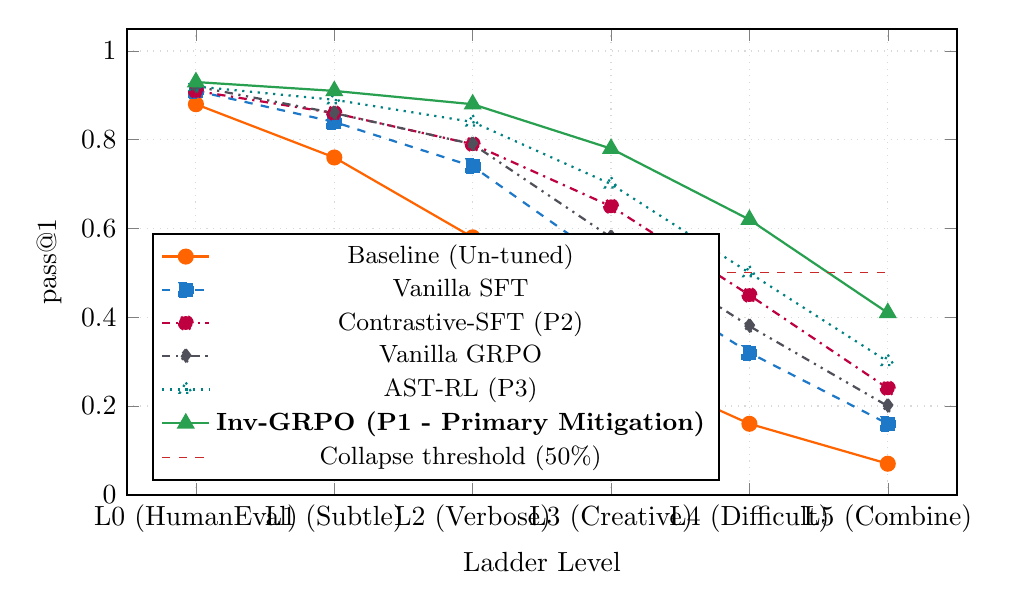
\begin{tikzpicture}
\begin{axis}[
  width=\textwidth, height=7.5cm,
  xlabel={Ladder Level}, ylabel={pass@1},
  xtick={0,1,2,3,4,5},
  xticklabels={L0 (HumanEval), L1 (Subtle), L2 (Verbose), L3 (Creative), L4 (Difficult), L5 (Combine)},
  ymin=0, ymax=1.05,
  grid=both, grid style={dotted, gray!30},
  legend pos=south west,
  legend style={font=\small},
  thick,
]
% Baseline (sharp collapse)
\addplot[OrangeMain, mark=*, mark size=2.5] coordinates {
  (0,0.88)(1,0.76)(2,0.58)(3,0.30)(4,0.16)(5,0.07)
};
\addlegendentry{Baseline (Un-tuned)}

% Vanilla SFT
\addplot[AccentBlue, mark=square*, mark size=2.5, dashed] coordinates {
  (0,0.91)(1,0.84)(2,0.74)(3,0.52)(4,0.32)(5,0.16)
};
\addlegendentry{Vanilla SFT}

% Contrastive-SFT (P2)
\addplot[purple, mark=otimes*, mark size=2.5, dashdotted] coordinates {
  (0,0.91)(1,0.86)(2,0.79)(3,0.65)(4,0.45)(5,0.24)
};
\addlegendentry{Contrastive-SFT (P2)}

% Vanilla RLVR
\addplot[MidGray, mark=diamond*, mark size=2.5, dashdotdotted] coordinates {
  (0,0.92)(1,0.86)(2,0.79)(3,0.58)(4,0.38)(5,0.20)
};
\addlegendentry{Vanilla GRPO}

% AST-RL (P3)
\addplot[teal, mark=triangle, mark size=2.5, dotted] coordinates {
  (0,0.92)(1,0.89)(2,0.84)(3,0.70)(4,0.50)(5,0.30)
};
\addlegendentry{AST-RL (P3)}

% Inv-GRPO (P1 - Ours)
\addplot[SuccessGreen, mark=triangle*, mark size=3.0] coordinates {
  (0,0.93)(1,0.91)(2,0.88)(3,0.78)(4,0.62)(5,0.41)
};
\addlegendentry{\textbf{Inv-GRPO (P1 - Primary Mitigation)}}

% 50% threshold
\addplot[AlertRed, dashed, thin] coordinates {(0,0.5)(5,0.5)};
\addlegendentry{Collapse threshold (50\%)}
\end{axis}
\end{tikzpicture}
\caption{Comparative performance degradation curves across the Reduction Ladder, illustrating how each prioritized mitigation arm delays the collapse point towards L4/L5.}
\label{fig:expected_results}
\end{figure}

%============================================================
\section{Multi-Dimensional Evaluation Metrics}
%============================================================

\begin{table}[H]
\centering
\caption{Complete evaluation metric suite with mathematical formulations}
\label{tab:metrics}
\renewcommand{\arraystretch}{1.4}
\begin{tabularx}{\textwidth}{l l X}
\toprule
\textbf{Metric} & \textbf{Mathematical Formulation} & \textbf{Scientific Purpose} \\
\midrule
Pass@1 & $p_1 = \frac{1}{|D|} \sum_{i=1}^{|D|} \mathbb{I}(\text{sample}_1 == \text{PASS})$ & Primary greedy accuracy ($T=0.0$). \\
Pass@5 & $p_5 = 1 - \frac{\binom{n-c}{5}}{\binom{n}{5}}$ & Exploration coverage across 5 samples ($T=0.8$). \\
Collapse Point & $\ell^* = \min \{ \ell \mid \text{pass@1}(\ell) < 0.50 \}$ & Threshold of catastrophic failure. \\
Ladder AUC & $\mathcal{A} = \frac{1}{6} \sum_{\ell=0}^{5} \text{pass@1}(\ell)$ & Aggregate gracefulness of degradation. \\
Consistency Delta & $\Delta_c = |\text{pass@1}(L_1) - \text{pass@1}(L_2)|$ & Sensitivity to surface-level lexical variations. \\
Memorisation Risk & $\text{MRI} = \text{Sim}(y, y^*) \cdot \max(0, p_1(L_0) - p_1(L_3))$ & Quantitative score for harmful memorisation~\cite{memorize_or_generalize}. \\
Token Efficiency & $\tau_\ell = \text{Mean}(\text{Length}(\text{Reasoning Tokens}))$ & Trace dynamics across difficulty levels. \\
\bottomrule
\end{tabularx}
\end{table}

%============================================================
\section{Repository Architecture \& Hardware Feasibility}
%============================================================

\begin{lstlisting}[style=pythonstyle, caption={Repository layout for reproduction}]
reduction-ladder-for-code/
|-- config.yaml                 # Central hyperparameter configuration
|-- proposal/                   # LaTeX proposal & references
|-- data/ladder/                # Standardized L0-L5 benchmark JSONL files
|-- src/
|   |-- data_pipeline/          # Benchmark loader & sandbox verifier
|   |-- evaluation/             # Execution harness & error classifier
|   |-- distillation/           # SFT positive & contrastive datasets
|   |-- training/               # QLoRA, Contrastive SFT, GRPO, Inv-GRPO
|   `-- analysis/               # Metric computers & publication plots
|-- notebooks/                  # 5 sequential Jupyter notebooks
`-- scripts/                    # Command-line entry points (run_stage*.py)
\end{lstlisting}

\begin{table}[H]
\centering
\caption{Hardware requirements and VRAM budget (RTX 3070 / 8GB VRAM)}
\label{tab:hardware}
\renewcommand{\arraystretch}{1.35}
\begin{tabularx}{\textwidth}{l l X}
\toprule
\textbf{Stage} & \textbf{VRAM Budget} & \textbf{Optimization Strategy} \\
\midrule
Inference (Eval) & $\approx$ 4.0 GB & 4-bit NF4 precision, batch size 1 \\
QLoRA / Contrastive SFT & $\approx$ 6.5 GB & PEFT LoRA adapters, gradient accumulation = 4 \\
GRPO / AST-RL / Inv-GRPO & $\approx$ 7.2 GB & Gradient checkpointing, group size $G=4$ \\
\bottomrule
\end{tabularx}
\end{table}

\begin{table}[H]
\centering
\caption{Project risk register and mitigations}
\renewcommand{\arraystretch}{1.4}
\begin{tabularx}{\textwidth}{l c c X}
\toprule
\textbf{Risk} & \textbf{Prob.} & \textbf{Impact} & \textbf{Mitigation Strategy} \\
\midrule
VRAM OOM during Inv-GRPO & Med & Med & Enable gradient checkpointing; interleave prompt-pair generation \\
Benchmark format mismatch & Low & Low & Automated schema normalization in Stage 1 \\
AST Parsing Failures & Low & Low & Fallback to execution reward if syntax tree generation fails \\
\bottomrule
\end{tabularx}
\end{table}

%============================================================
\section{Timeline \& Orange Innovation Deliverables}
%============================================================

\begin{table}[H]
\centering
\caption{Project timeline (12 weeks)}
\label{tab:timeline}
\renewcommand{\arraystretch}{1.5}
\begin{tabularx}{\textwidth}{c l X l}
\toprule
\textbf{Weeks} & \textbf{Stage} & \textbf{Key Research Activities} & \textbf{Deliverables} \\
\midrule
1--2 & \textcolor{OrangeMain}{\textbf{S1}} Benchmark Ingestion & Ingest & validate L0--L5 benchmarks & Normalized JSONL datasets \\
3--4 & \textcolor{OrangeMain}{\textbf{S2}} Baseline Eval & Full ladder evaluation of un-tuned Qwen-1.5B & Baseline results \& $\ell^*$ \\
5--6 & \textcolor{OrangeMain}{\textbf{S3}} SFT Arms & Train Vanilla SFT vs Contrastive-SFT (P2) & SFT Checkpoints \\
7--9 & \textcolor{OrangeMain}{\textbf{S4}} RL Arms & Train Vanilla GRPO vs AST-RL (P3) vs Inv-GRPO (P1) & RL Checkpoints \\
10--12 & \textcolor{OrangeMain}{\textbf{S5}} Synthesis & Multi-arm comparative curves, Error Taxonomy, Report & Final Report \& Codebase \\
\bottomrule
\end{tabularx}
\end{table}

%============================================================
% REFERENCES
%============================================================
\newpage
\printbibliography[title={References}]

\end{document}